\section{Cross Sections}
\label{sec:cross_sections}

We introduce a new method of origami construction, using cross section disgrams.
Instead of beginning our construction from a 2-dimensional sheet of paper,
we consider a 1-dimensional cross section moving forwards in time.
A simple example is demonstrated in Figure~\ref{fig:strip_narrowing}.

\todo[inline]{Conservation of length}
\section{Segments and Cross Sections}
\label{sec:segments_and_cross_sections}

\begin{definition}
\label{def:segment}
A segment $s$ is an oriented line segment with left and right endpoints $\vec s_l$ and $\vec s_r$.
Each segment is also associated with an orientation vector $\vec{\hat o_s} \equiv\frac{\vec s_r-\vec s_l}{ \left\| \vec s_r-\vec s_l\right\|}$.
This vector serves to disambiguate the orientation of zero length segments.
\end{definition}

\begin{definition}
\label{def:cross_section}
A cross section $C$ is defined as an ordered list of line segments $\langle s_1,s_2,\cdots,s_n\rangle$,
such that for every segment $s_i$ (except the last),
the right endpoint of $s_i$ coincides with the left endpoint of $s_{i+1}$.
Each segment $s$ is also associated with a velocity vector $\vec{\hat v_s}$ of unit magnitude.
For a segment $s\in C$ we will also denote this velocity as $\vec{\hat v_i}$.
\end{definition}

\begin{definition}
\label{def:node}
Given a cross section $C = \langle s_1, s_2,\cdots s_n \rangle$, a node $x$ denotes a point on one of the segments $s_i$.
A joint node is a node that resides on the endpoint of a segment.
The distance between two nodes on a cross section is defined as the overall length f cross section between the two nodes.
\todo[inline]{Distance}
\end{definition}

\begin{restatable}{pro}{UniformVelocity}
\label{pro:uniform_velocity}
All nodes on a segment $s$ except the joint nodes move with the same velocity $\vec{\hat v_s}$.
\end{restatable}

\begin{restatable}{pro}{OrthogonalVelocity}
\label{pro:orthogonal_velocity}
The velocity $\vec{\hat v_s}$ of segment $s$ is orthogonal to its orientation $\vec{\hat o_s}$.
\end{restatable}

\subsection{Joints}
\label{sec:joints}

\begin{definition}
\label{def:joints}
A cross section with $n$ segments is also associated with a list of joints
$ \langle J_1,\cdots J_{n-1} \rangle$, where $J_i$ corresponds to the right endpoint of $s_i$.
The velocity of a joint $J_i$, is $\vec J_v = \vec v_i+\vec v_{i+1}$
(i.e. the sum of the velocities of the corresponding segments).
\end{definition}
\begin{definition}
\label{def:creases}
Note that the trajectory of the joints form a crease \ldots angle is angle between direction vectors.
Creases are also created when a segment changes direction\ldots angle is change in direction vector.
\end{definition}

\begin{definition}
\label{def:joint_plane}
A joint plane is the plane that coincides with both segments $l$ and $r$ associated with a particular joint $J$.
\end{definition}

\begin{definition}
\label{def:joint_plane_velocity}
Consider a joint $J$ associated with segments $l$ and $r$, and joint plane $\mathcal P$,
where $\vec v_l$ and $\vec v_r$ are the velocities of segments $l$ and $r$.
We define $\vec v_l^\shortparallel$ and $\vec v_l^\perp$ as the components of $\vec v_l$ coinciding with,
and orthogonal to the joint plane respectively.
Similarly, we define $\vec v_r^\shortparallel$ and $\vec v_r^\perp$, as the components of $\vec v_r$.
Further, note that $\vec v_l^\shortparallel$ and $\vec v_r^\shortparallel$
have to be orthogonal to $\vec o_l$ and $\vec o_r$ respectively.
\end{definition}

\begin{claim}
\label{clm:joint_orthogonal_velocity}
For a joint $J$ associated with segments $l$ and $r$, $\vec v_l^\perp = \vec v_r^\perp$.
\end{claim}

\begin{corollary}
\label{cor:joint_plane_velocity}
For a joint $J$ associated with segments $l$ and $r$,
$ \left\| \vec v_l^\shortparallel\right\| = \left\| \vec v_r^\shortparallel\right\|$.
\end{corollary}

\begin{claim}
\label{clm:valid_joint}
A joint $J$ corresponding to segments $s$ and $t$ is \emph{valid}
if the resulting evolution of the joint preserves distances.
\end{claim}

\subsection{Time Travel}
\label{sec:time_travel}

In the process of time travel, all the nodes on a segment $s$, except the
\emph{joint nodes} move with velocity $\vec{\hat v}_s$ (orthogonal to $\vec{\hat
o_s}$). For example, if we allow a single segment of length $X$ to evolve for
time $T$, it will result in a $X\times T$ strip of paper.

The joint node velocity $\vec J_v$ may have a component along a corresponding
segment $s$ (along $\vec{\hat o}_s$). As a result, the lengths of segments may
change (Figure~\ref{fig:trapezoid_angles}). This can be visualized as movement
of the corresponding joint along one of the segments.

\begin{definition}
\label{def:segment_length}
For every segment $s$ in a cross section $C$, we associate a left pace $L_s$,
which indicates the rate at which $s$ shrinks from its left endpoint.
Similarly, we define a right pace $R_s$ grows from its right endpoint.
Note that both these quantities can be negative.
\end{definition}
After time $T$, the length of a segment changes by $T\cdot(R_s-L_s)$.
The length of a segment is not allowed to become negative.
For a segment $s_i$ with left joint $J^L$ and right joint $J^R$, we obtain the relations
\begin{align*}
\vec J_v^L-\vec{\hat v_{s_i}} = L_{s_i}\cdot \vec{\hat o_{s_i}}, && \vec J_v^R-\vec{\hat v_{s_i}} = R_{s_i}\cdot \vec{\hat o_{s_i}}.
\end{align*}

\begin{definition}
\label{def:valid_joint}
A joint $J$ corresponding to segments $s$ and $t$ is \emph{valid} if and only if the evolution
resulting from the velocities $\vec{\hat v}_l$, $\vec{\hat v}_r$, and $\vec J_v$ preserves distances between the non-joint nodes.
\end{definition}
\vspace{-1pc}
\begin{restatable}{inv}{LeftRightPace}
\label{inv:left_right_pace}
The right pace of $s_{i}$ is equal to the left pace of $s_{i+1}$.
This is to preserve the overall length of the cross section, and the distance between any two nodes.
Furthermore, the left pace of the first segment, and the right pace of the last segment should be zero, i.e., $L_0 = R_n = 0$
This ensures that the total length of the cross section does not change.
\end{restatable}

The movement of a joint increases the length of one of its associated segments,
and decreases the length of the other segment by the same amount (this ensures that the total length is preserved).
This puts some constraints on the possible velocities of adjacent segments.

Consider a joint $\vec J_i$ corresponding to segments $l = s_i$ and $r = s_{i+1}$, at time $t=0$.
Henceforth, we will refer to $L_r$ as $L$, and $R_l$ as $R$.
Without loss of generality, we assume that $L<0$.
At a later time $t$, let the new joint position be $\vec J'_i$.
We define nodes $a$ and $b$ corresponding to $\vec J_i$ and $\vec J_{i+1}$ respectively.
We also define the initial and final positions of $a$ as $\vec a$,
and $\vec a'$, and similarly for $b$, we define $\vec b$ and $\vec b'$.
Let $d$ be the \emph{separation} between nodes $a$ and $b$.
This setup is shown in Figure~\ref{fig:joint_plane_velocity}.

%\begin{figure}[htpb]
\begin{wrapfigure}[8]{r}{0.4\textwidth}
%\vspace{-2.2em}
\graphicspath{{./notebooks/}}
    \centering
    \def\svgwidth{\linewidth}
    \input{notebooks/joint_plane_velocity.pdf_tex}
    \caption{A joint with segments $l$ and $r$.
    The trajectory of the joint is shown in orange.
    The trajectories of $a$ and $b$ are shown in blue.
    The green arrows indicate $\vec v^\shortparallel$.}
    \label{fig:joint_plane_velocity}
\end{wrapfigure}
%\end{figure}


First, note that $\vec a, \vec b$ lie on the segment $l$, and $\vec a', \vec b'$ lie on the segment $r$,
which implies that $\vec b-\vec a = d\cdot \vec{\hat o}_l$, and $\vec b'-\vec a' = d\cdot \vec{\hat o}_r$:
\begin{align*}
\vec b' - \vec a' &= (\vec b + t\cdot \vec{\hat v}_r^\shortparallel) - (\vec a + t\cdot \vec{\hat v}_l^\shortparallel)\\
\implies \vec b' - \vec a' &= (\vec b - \vec a) + t\cdot(\vec{\hat v}_r^\shortparallel - \vec{\hat v}_l^\shortparallel)\\
\implies d\cdot \vec{\hat o}_r &= d\cdot \vec{\hat o}_l + t\cdot(\vec{\hat v}_r^\shortparallel - \vec{\hat v}_l^\shortparallel)\\
\implies \vec{\hat v}_r^\shortparallel - \vec{\hat v}_l^\shortparallel &= \frac{d}{t}\cdot(\vec{\hat o}_r-\vec{\hat o}_l)
= -R\cdot(\vec{\hat o}_r-\vec{\hat o}_l)
\\&  % line break for narrow column
= -L\cdot(\vec{\hat o}_r-\vec{\hat o}_l).
\end{align*}
This is only possible if $\vec{\hat o}_l\times \vec{\hat o}_r$ is oriented opposite to $\vec{\hat v}_l^\shortparallel\times \vec{\hat v}_r^\shortparallel$.

\begin{restatable}{inv}{SegmentOrientation}
\label{inv:SegmentOrientation}
Given two adjacent segments $l$ and $r$ in a cross section $C$, the vector
$\vec{\hat o}_l\times \vec{\hat o}_r$ must be oriented opposite to $\vec{\hat v}_l^\shortparallel\times \vec{\hat v}_r^\shortparallel$.
\end{restatable}

If the angle between the segments (between $\vec{\hat o}_l$ and $\vec{\hat o}_r$) is $\theta$,
the magnitude of $\vec{\hat o}_r-\vec{\hat o}_l$ is $\sqrt{2-2\cos(\theta)}$,
and $ \left\| \vec{\hat v}_r^\shortparallel-\vec{\hat v}_l^\shortparallel\right\| = v\cdot\sqrt{2-2\cos(\pi-\theta)}$.
Here, $v$ is magnitude of the plane velocity (projection onto the joint plane
$\mathcal P$) of $\vec J_i$.
Given $\omega = \theta/2$, we get --
\begin{align*}
-L = -R &= \frac dt = \vec{\hat v}_l - \vec{\hat o}_l\frac{ \left\| \vec{\hat v}_r^\shortparallel
- \vec{\hat v}_l^\shortparallel\right\|}{ \left\| \vec{\hat o}_r-\vec{\hat o}_l\right\|}
= v\cdot\frac{\sqrt{\sin^2\left( {\pi/2-\theta/2}\right)}}{\sqrt{\sin^2{\theta/2}}}
= v\cdot\cot\left( \omega \right).
\end{align*}

\begin{restatable}{inv}{JointVelocity}
\label{inv:joint_velocity}
The velocity of a joint $J$ associated with segments $l$ and $r$, is a constant vector
$\vec J_v
%= \vec{\hat v}_l - \vec{\hat o}_l\frac{ \left\| \vec{\hat v}_r^\shortparallel
%- \vec{\hat v}_l^\shortparallel\right\|}{ \left\| \vec{\hat o}_r-\vec{\hat o}_l\right\|}
= \vec{\hat v}_l - \left\| \vec{\hat v}_l^\shortparallel\right\|\cdot\vec{\hat o}_l\cdot\cot\left( \theta/2 \right)$,
where $\theta$ is the angle between $\vec{\hat o}_l$ and $\vec{\hat o}_r$.
\end{restatable}

%\todo[inline]{
%Note that time evolution is reversible.
%}

\subsection{Cross Section Interval Folding}
\label{sec:interval_folding}

\begin{definition}
\label{def:interval}
We consider a cross section $C$ composed of segments $ \langle s_1,s_2,\cdots,s_n \rangle$
with total length $X$ (i.e. $\sum \left| s_i\right| = X$).
If we allow this cross section to evolve for time $T$, we obtain a new cross section $C_T = \langle r_1,r_2,\cdots ,r_n \rangle$.
The evolution from $C$ to $C_T$ forms a cross section interval $\mathcal C$ of length $T$.
\end{definition}

\begin{definition}
\label{def:}
Say that the total length of the cross sections in $\mathcal C$ is $X$ (we showed in \ldots that length is conserved).
We will denote a strip of paper of size $X\times L$ as an $L$-strip.
\end{definition}

\subsubsection{Interval Folding results in Flat Strip}
\label{sec:interval_flat_strip}

In this section, we focus on a single cross section interval $\mathcal C$ with segments $\langle s_1, s_2,\cdots s_n \rangle$ evolving over time $T$.
First consider the surface traced out by an individual segment $s_i$.
Since the endpoints of $s_i$ move in a straight line, each segment traces \todo{What is a trace?} a trapezoid.

\begin{figure}[htb]
\graphicspath{{./figures/}}
    \centering
    \subfloat[] {
        \def\svgwidth{0.5\textwidth}
        \input{figures/trapezoid.pdf_tex}
        \label{fig:segment_trapezoid}
    }
    \hspace{-9em}
    \subfloat[] {
        \def\svgwidth{0.7\textwidth}
        \input{figures/trapezoid_angles.pdf_tex}
        \label{fig:trapezoid_angles}
    }
    \caption{}
    \label{fig:trapezoids}
\end{figure}

\begin{definition}
\label{def:interval_folding}
Given a cross section interval $\mathcal C$ formed from a cross section $C$ evolving over time $T$,
we define the folding of $\mathcal C$ as the surface swept out by $C$ from over time $T$.
Precisely
\begin{enumerate}
\item The folding of a the $i^{th}$ segment is the trapezoid formed by the initial and final state of the segment ($s_i$ and $r_i$).
      This forms a trapezoid of height $T$ (Figure~\ref{fig:segment_trapezoid}).
      The non-parallel sides are straight lines due to Property~\ref{pro:joint_velocity}.
      In case either the initial or final segment has length, the resulting trapezoid will be a triangle.
\item For every joint $J_i$, we attach the corresponding trapezoids for $s_i$ and $s_{i+1}$
      along the joint trajectory $\mathcal T_{J_i}$ to obtain the folding of $\mathcal C$.
\end{enumerate}
\end{definition}

First, we will show that each $\mathcal C_i$ corresponds to a $T_i$-strip.

\begin{definition}
\label{def:trapezoid}
The surface traced out by a segment $s$ is a trapezoid $Z_s$ (Figure~\ref{fig:segment_trapezoid}).
Specifically, if $L,R$ are the initial left and right endpoints of $s$, and $L',R'$ are the final endpoints,
$Z_s = LL'R'R$ is the corresponding trapezoid (Figure~\ref{fig:segment_trapezoid}).
\end{definition}

\todo[inline]{Define gluing}

\begin{lemma}
\label{lem:trapezoid_gluing_parallel}
Consider a joint $J$ with segments $l$ and $r$, which has zero orthogonal joint velocity (i.e. $\vec v_l^\shortparallel = \vec v_r^\shortparallel = 0$.
The gluing of trapezoids $Z_l$ and $Z_r$ along the joint trajectory $\mathcal T_J$ is isometric to a larger trapezoid.
This joint trajectory is actually nothing but a crease in the folded state.
\end{lemma}

\begin{figure}[!htb]
\graphicspath{{figures/trapezoidZ}}
    \centering
    %\subfloat[]{
        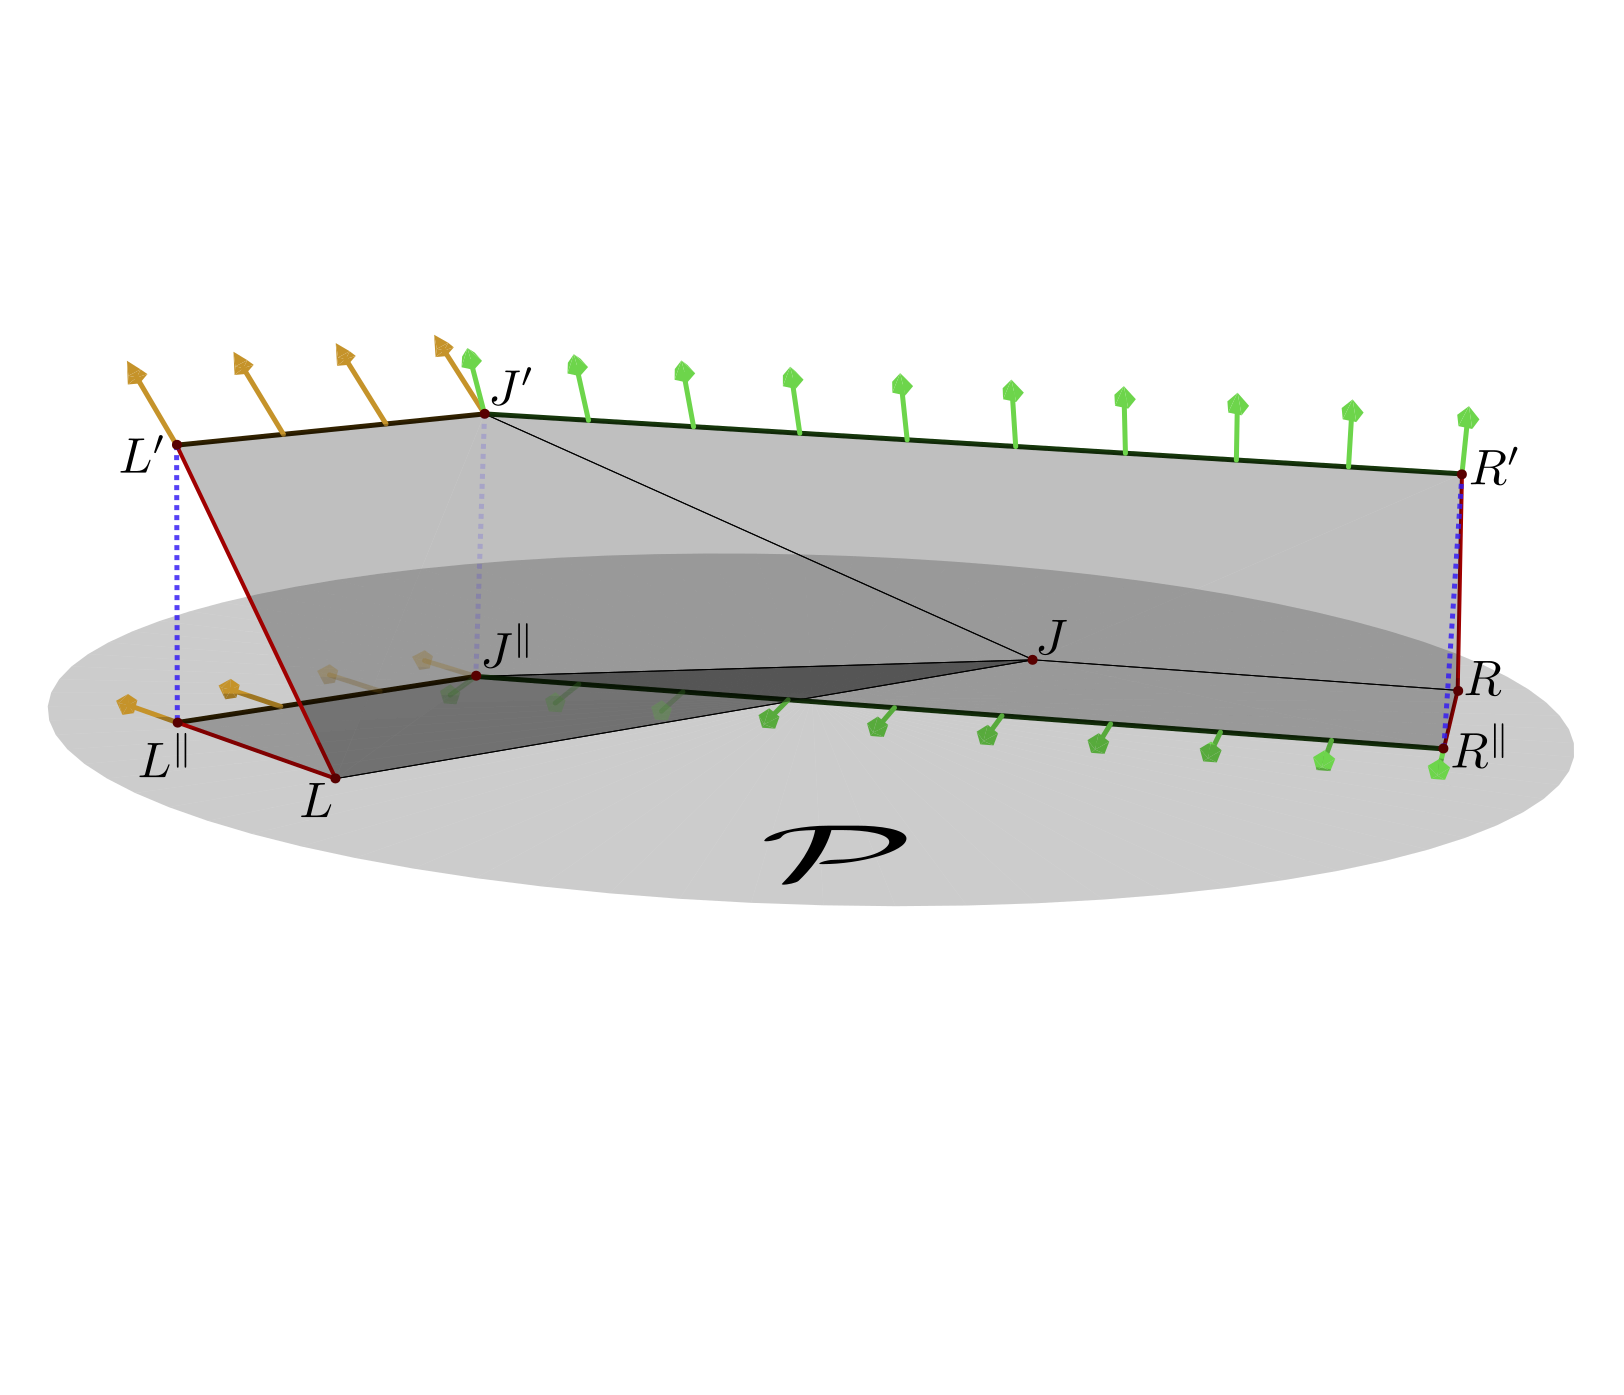
\includegraphics[width=0.5\textwidth]{figures/trapezoidZ/trapezoidZ0.pdf}%
    %}%
    %\subfloat[]{
        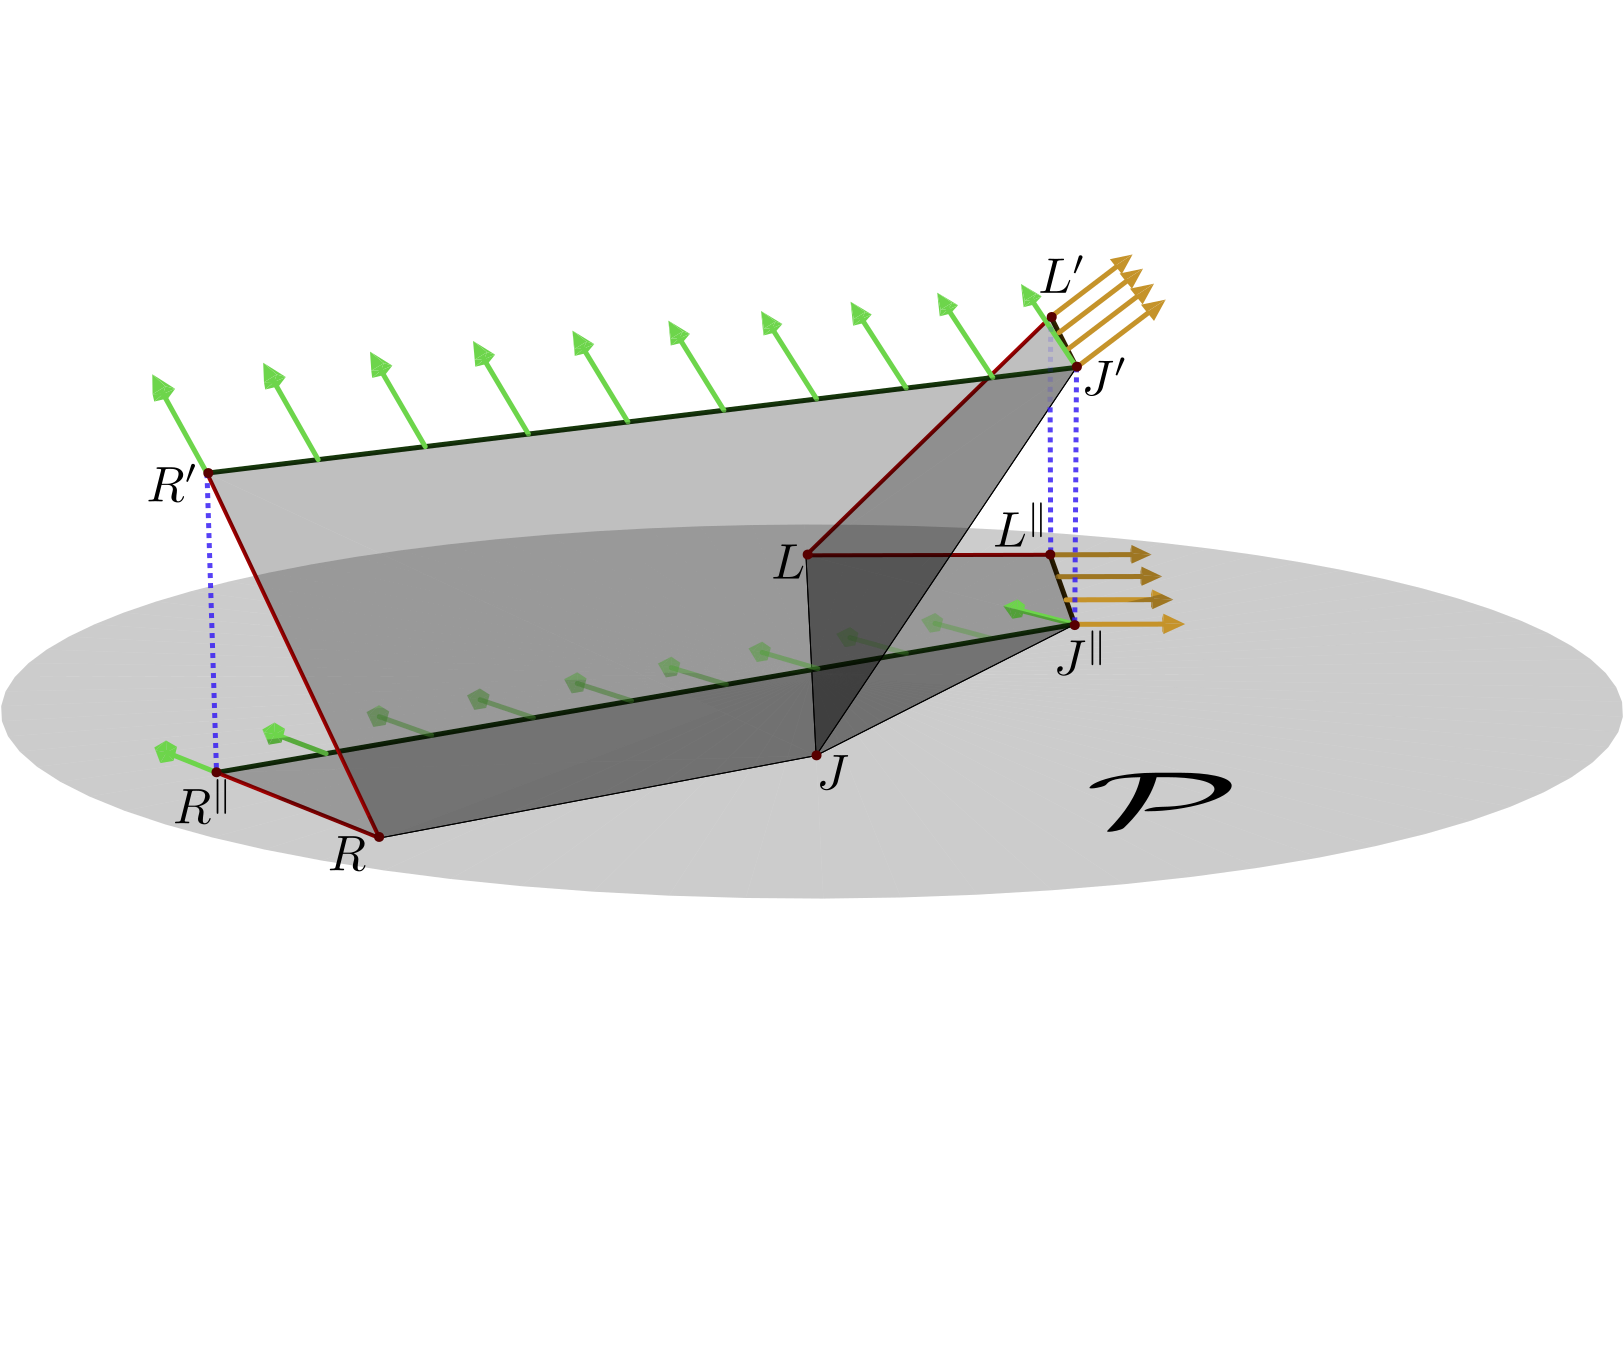
\includegraphics[width=0.5\textwidth]{figures/trapezoidZ/trapezoidZ1.pdf}%
    %}%

    %\subfloat[]{
        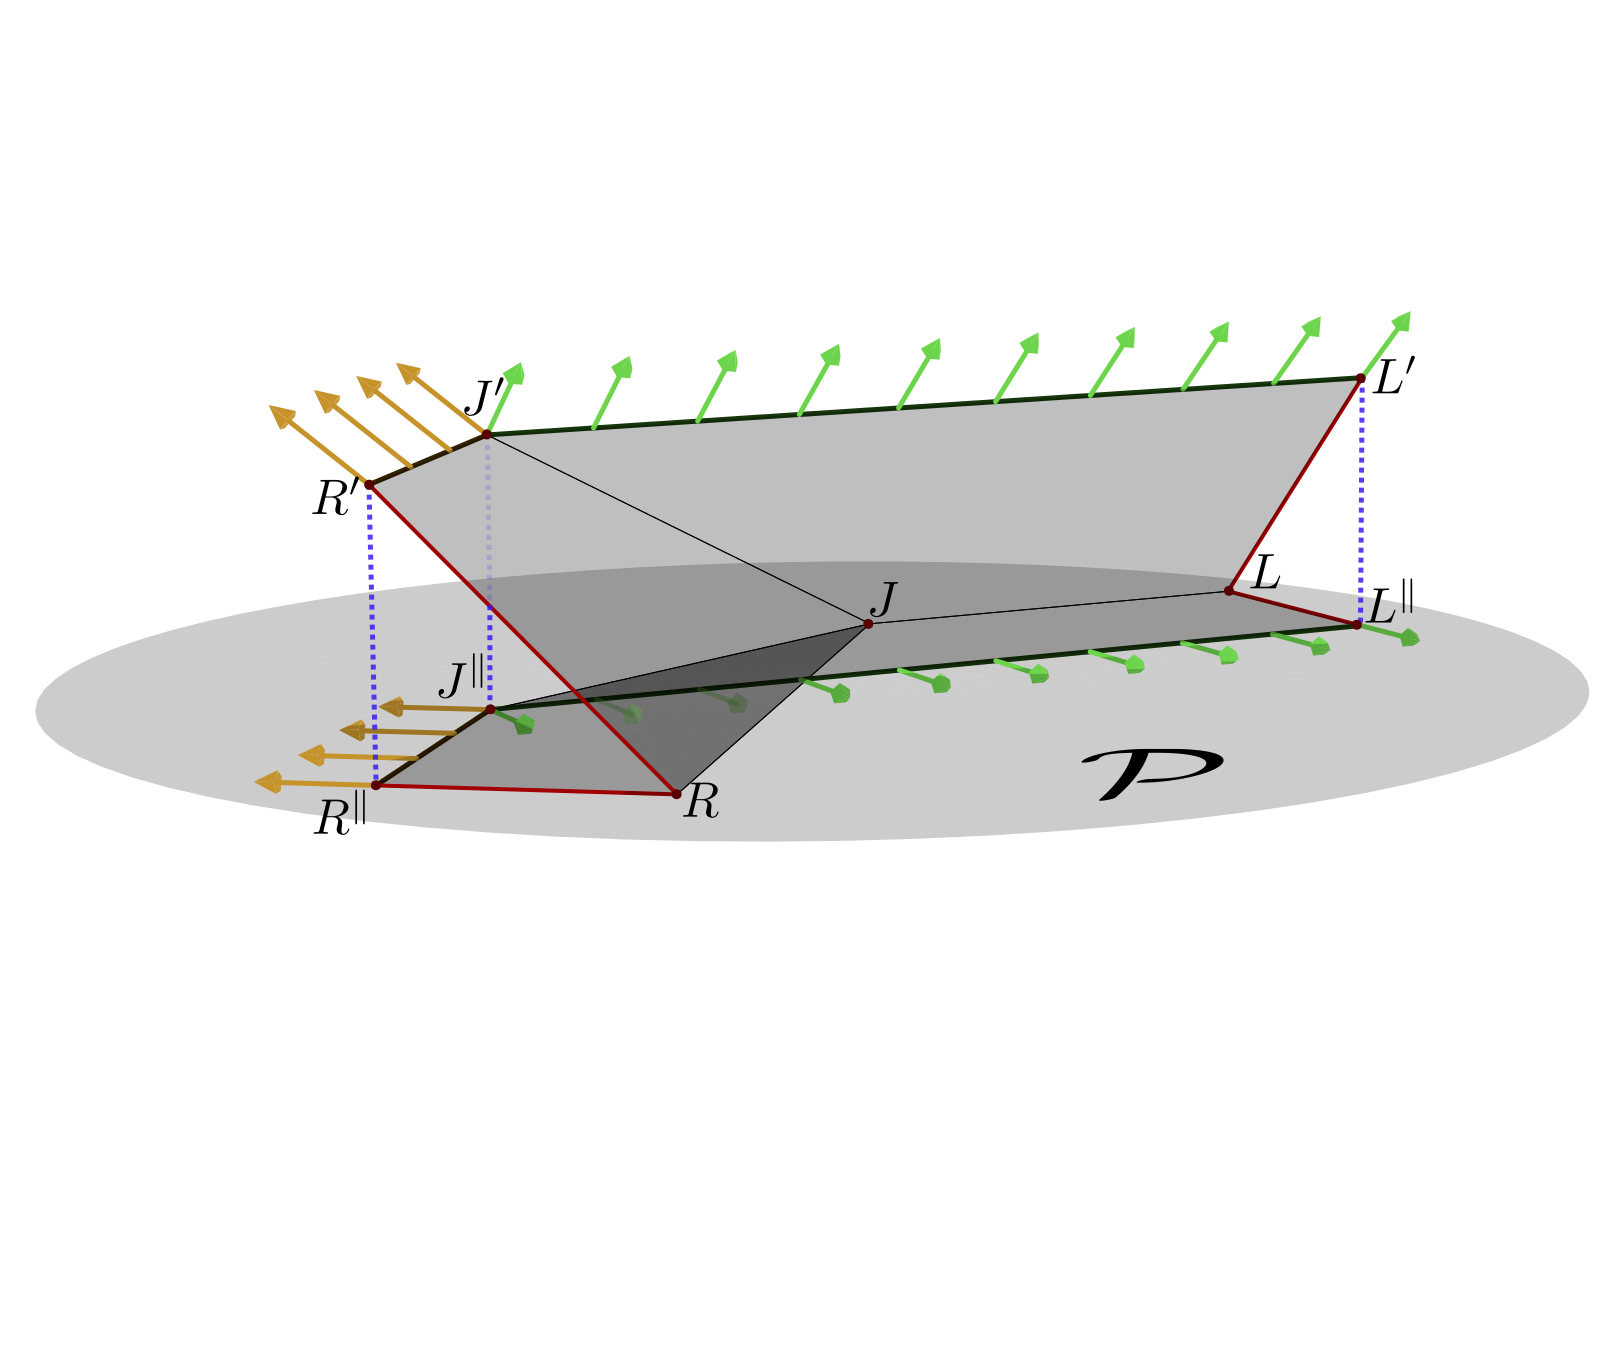
\includegraphics[width=0.8\textwidth]{figures/trapezoidZ/trapezoidZ2.pdf}%
    %}%
    \caption{
    Evolution of a joint with non-zero orthogonal velocity from $LJR$ to $L'J'R'$.
    The blue dotted lines represent the projection of the final state to the joint plane $\mathcal P$.
    }
    \label{fig:trapezoidZ}
\end{figure}

\begin{lemma}
\label{lem:trapezoid_gluing}
Consider a joint $J$ with segments $l$ and $r$ with non-zero orthogonal velocity.
The gluing of trapezoids $Z_l$ and $Z_r$ along the joint trajectory $\mathcal T_J$ is isometric to a larger trapezoid.
\end{lemma}
\begin{proof}
As before, let $LJR$ and $L'J'R'$ represent the initial and final positions of the segments respectively.
We also construct the projection of $L'J'R'$ to the joint plane $\mathcal P$ as $L^\shortparallel J^\shortparallel R^\shortparallel$.
The evolution of the projection is analogous to the setting in Lemma~\ref{lem:trapezoid_gluing_parallel}.
Therefore, $\angle LJJ^\shortparallel = \phi = \theta/2$ and $\angle RJJ^\shortparallel = \pi-\phi$.

Consider the positive $z$-axis along the joint orthogonal velocity (i.e. normal to the joint plane $\mathcal P$).
We define the orthogonal diaplacement vector as $\overrightarrow{JJ'} = z\cdot\vec{\hat k}$.
Let the positive $x$-axis be along $JJ^\shortparallel$. So, the unit vector along $\overrightarrow{JJ'}$ is $\frac{1}{\sqrt{1+z^2}}(1,0,z)$.

Since $\angle J^\shortparallel JR = \phi$, the unit vector along $\overrightarrow JR$ is $(\cos\phi,\sin\phi,0)$.
So, we compute $\cos \angle RJJ' = \cos\phi/\sqrt{1+z^2}$.
Similarly, since $\angle J^\shortparallel JL = \pi-\phi$, the unit vector along $\overrightarrow JL$ is $(-\cos\phi,\sin\phi,0)$,
which implies that $\cos \angle LJJ' = -\cos\phi/\sqrt{1+z^2}$.
Finally, since both $\angle LJJ$ and $\angle RJJ'$ are less than $\pi$, and $\cos\left(\angle LJJ' \right) = -\cos\left(\angle RJJ' \right)$,
we conclude that $\angle LJJ' + \angle RJJ' = \pi$.

Since $LJJ'L'$ and $RJJ'R'$ are both trapezoids, this implies that the resulting gluing along $JJ'$ is a larger trapezoid.
\end{proof}

\begin{theorem}
\label{thm:interval_strip}
Consider a cross section interval $\mathcal C$ formed from a cross section $C$ evolving over time $T$ to form a folding $F$.
Further assume that the total length of cross section $C$ is $X$ units. Then, $F$ is isometric to a $X\times T$ strip of paper.
\end{theorem}
\begin{proof}
From Lemma~\ref{lem:trapezoid_gluing}, we know that $F$ is isometric to a trapezoid.
Let $L,L'$ be the initial and final positions of the left (non-parallel) edge of the trapezoid, and
let $R,R'$ be the initial and final positions of the right edge of the trapezoid.
Say that $C$ comprises of segments $ \langle s_1, s_2,\cdots s_n \rangle$.
From Property~\ref{pro:left_right_velocity}, we know that the left velocity of $s_0$ is zero.
So, the line $LL'$ follows the trajectory of $\vec{\hat v_0}$, which is orthogonal to the segment $s_0$.
In other words, the left edge of the trapezoid has length $T$, and is orthogonal to the parallel edges.
Similarly, because the right velocity of $s_n$ is zero, the right edge of the trapezoid is also orthogonal.
Therefore, $F$ is isometric to a right angled trapezoid (i.e. a strip) of length $X$ and width $T$.
\end{proof}
\todo[inline]{property for NO zero length segments}


\subsection{Multiple Cross Sections}
\label{sec:intervals}
\graphicspath{{./figures/strip_narrowing/}}
\begin{figure}[!htb]
    \begingroup
    \def\svgwidth{0.23\textwidth}
        \captionsetup[subfigure]{width=0.22\textwidth}
        \subfloat[The trivial cross section.] {
        \input{figures/strip_narrowing/strip0.pdf_tex}
        }%
    \endgroup%
    \begingroup
    \def\svgwidth{0.23\textwidth}
        \captionsetup[subfigure]{width=0.48\textwidth}
        \subfloat[New zero length segment inserted at left endpoint. Existing segment reverses direction.] {
        \input{figures/strip_narrowing/strip10.pdf_tex}
        %}%
    %\endgroup%
    %\begingroup
    \def\svgwidth{0.23\textwidth}
        %\captionsetup[subfigure]{width=0.22\textwidth}
        %\subfloat[] {
        \input{figures/strip_narrowing/strip11.pdf_tex}
        }%
    \endgroup%
    \begingroup
    \def\svgwidth{0.23\textwidth}
        \captionsetup[subfigure]{width=0.22\textwidth}
        \subfloat[Evolution continues] {
        \input{figures/strip_narrowing/strip12.pdf_tex}
        }%
    \endgroup%
    \begingroup
    \def\svgwidth{0.23\textwidth}
        \captionsetup[subfigure]{width=0.67\textwidth}
        \subfloat[New zero length segment (red) inserted between two existing segments
                  with the same velocity as the rightmost segment.
                  Existing segments retain their direction.] {
        \input{figures/strip_narrowing/strip20.pdf_tex}
        %}%
    %\endgroup%
    %\begingroup
    \def\svgwidth{0.23\textwidth}
        %\captionsetup[subfigure]{width=0.22\textwidth}
        %\subfloat[] {
        \input{figures/strip_narrowing/strip21.pdf_tex}
        %}%
    %\endgroup%
    %\begingroup
    \def\svgwidth{0.23\textwidth}
        %\captionsetup[subfigure]{width=0.22\textwidth}
        %\subfloat[] {
        \input{figures/strip_narrowing/strip22.pdf_tex}
        }%
    \endgroup%
    %\begingroup
    %\def\svgwidth{0.23\textwidth}
        %\captionsetup[subfigure]{width=0.22\textwidth}
        %\subfloat[Evolution continues] {
        %\input{figures/strip_narrowing/strip23.pdf_tex}
        %}%
    %\endgroup%
    \begingroup
    \def\svgwidth{0.23\textwidth}
        \captionsetup[subfigure]{width=0.28\textwidth}
        \subfloat[Length of leftmost (blue) segment becomes zero.] {
        \input{figures/strip_narrowing/strip24.pdf_tex}
        }%
    \endgroup%
    \begingroup
    \def\svgwidth{0.23\textwidth}
        \captionsetup[subfigure]{width=0.48\textwidth}
        \subfloat[Leftmost (zero length) segment is deleted.
                  The remaining two segments continue in the same direction.
                  Overall strip width has been reduced] {
        \input{figures/strip_narrowing/strip30.pdf_tex}
        %}%
    %\endgroup%
    %\begingroup
    \def\svgwidth{0.23\textwidth}
        %\captionsetup[subfigure]{width=0.22\textwidth}
        %\subfloat[] {
        \input{figures/strip_narrowing/strip31.pdf_tex}
        }%
    \endgroup%
    \begingroup
    \def\svgwidth{0.48\textwidth}
        \captionsetup[subfigure]{width=0.44\textwidth}
        \subfloat[Side view of strip narrowing gadget, with layers separated. The red lines denote the boundaries of the cross section.] {
        \input{figures/strip_narrowing/strip_layers.pdf_tex}
        }%
    \endgroup%
        \caption{Cross section evolution of a strip narrowing gadget. \todo[inline]{cite} }
    \label{fig:strip_narrowing}
\end{figure}


\begin{definition}
\label{def:compatible}
Given two cross section intervals $\mathcal C$ and $\mathcal D$, such that $\mathcal C^F$ and $\mathcal D^I$ are equivalent,
we say that $\mathcal D$ is next-compatible with $\mathcal C$ and $\mathcal C$ is previous-compatible with $\mathcal D$.
Two cross sections $C = \langle s_1, s_2,\cdots s_n \rangle$ and $D = \langle r_1, r_2,\cdots r_m \rangle$ are equivalent
if and only if $C$ and $D$ correspond to the same sequence of segments after the deletion of all zero length segments.
\end{definition}

\begin{definition}
\label{def:cross_section_sequence}
A cross section sequence is a sequence is an ordered list of cross section intervals $ \langle \mathcal C_1, \mathcal C_2,\cdots \mathcal C_n \rangle$,
such that $C_{i}$ is next-compatible with $C_{i-1}$ for all $i\in [n-1]$.
This is equivalent to stating that $C_{i}$ is previous-compatible with $C_{i+1}$ for all $i\in [n-1]$.
Note that wedo not care about the directions of the segments.
\end{definition}

We will represent our full construction as a valid \emph{cross section sequence}.
Given a cross section sequence $\langle \mathcal C_1, \mathcal C_2,\cdots \mathcal C_n \rangle$,
the transition from $\mathcal C_i$ to $\mathcal C_{i+1}$ corresponds to the deletion of one or more
length zero segments from $\mathcal C_i$, and the addition of one or more zero length segments to obtain $\mathcal C_{i+1}$.
One simple example is shown in Figure~\ref{fig:strip_narrowing}.

\begin{definition}
\label{def:sequence_folding}
Given a cross section sequence $\langle \mathcal C_1, \mathcal C_2,\cdots \mathcal C_n \rangle$,
We obtain $\mathcal F_i$ as the folding of cross section $\mathcal C_i$.
the transition from $\mathcal C_i$ to $\mathcal C_{i+1}$ corresponds to the deletion of one or more
For every joint $J_i$, we attach the corresponding trapezoids for $s_i$ and $s_{i+1}$
along the joint trajectory to obtain the folding of $\mathcal C$.
\end{definition}

\subsubsection{Evolution Corresponds to Flat Paper}
\label{sec:flat}

In this section we will demonstrate that the folding formed by cross section evolution is realizable from a sheet of flat paper.
We note here that our construction may still result in self intersections.

We consider a cross section sequence $\langle \mathcal C_1, \mathcal C_2,\cdots \mathcal C_n \rangle$,
where each cross section interval $\mathcal C_i$ has evolution time $T_i$.

We will then use Theorem~\ref{def:cross_section_sequence} to attach the sequence of $T_i$-strips,
to form a complete $X\times T$ sheet of paper, where $T = \sum T_i$.

\begin{restatable}{thm}{main}
\label{thm:main}
Consider a cross section sequence $\langle \mathcal C_1, \mathcal C_2,\cdots \mathcal C_n \rangle$ where each
cross section interval $\mathcal C_i$ evolves over time $T_i$ to form a folding $F_i$ such that the following properties hold
\begin{itemize}
    \item[] \vspace{-2em}\OrthogonalVelocity*
    \item[] \vspace{-2em}\JointOrthogonalVelocity*
    \item[] \vspace{-2em}\LeftRightVelocity*
    \item[] \vspace{-2em}\JointVelocity*
\end{itemize}
Then, $F$ is isometric to a $X\times T$ strip strip of paper, where let $T = \sum T_i$.
\end{restatable}
\begin{proof}

\end{proof}

%\subsection{Evolution Corresponds to Flat Paper}
\label{sec:flat}

In this section we wil demonstrate that the folding formed by cross section evolution is realizable from a sheet of flat paper.
We note here that our construction may still result in self intersections.

We consider a cross section sequence $\langle \mathcal C_1, \mathcal C_2,\cdots \mathcal C_n \rangle$,
where each cross section interval $\mathcal C_i$ has evolution time $T_i$.
Say that the length ogf each cross section in the sequence is $X$.
We will denote a strip of paper of size $X\times L$ as an $L$-strip.

First, we will show that each $\mathcal C_i$ corresponds to a $T_i$-strip.
We will then use Theorem~\ref{def:cross_section_sequence} to attach the sequence of $T_i$-strips,
to form a complete $X\times T$ sheet of paper, where $T = \sum T_i$.

\subsubsection{Cross Section Interval Forms a Strip from a Gluing of Trapezoids}
\label{sec:cross_section_interval_strip}

In this section, we focus on a single cross section interval $\mathcal C$ with segments $\langle s_1, s_2,\cdots s_n \rangle$ evolving over time $T$.
First consider the surface traced out by an individual segment $s_i$.
Since the endpoints of $s_i$ move in a straight line, each segment traces \todo{What is a trace?} a trapezoid.

\begin{figure}[htb]
\graphicspath{{./figures/}}
    \centering
    \subfloat[] {
        \def\svgwidth{0.5\textwidth}
        \input{figures/trapezoid.pdf_tex}
        \label{fig:segment_trapezoid}
    }
    \hspace{-9em}
    \subfloat[] {
        \def\svgwidth{0.7\textwidth}
        \input{figures/trapezoid_angles.pdf_tex}
        \label{fig:trapezoid_angles}
    }
    \caption{}
    \label{fig:trapezoid}
\end{figure}

\begin{definition}
\label{def:trapezoid}
The surface traced out by a segment $s$ is a trapezoid $Z_s$ (Figure~\ref{fig:segment_trapezoid}).
Specifically, if $L,R$ are the initial left and right endpoints of $s$, and $L',R'$ are the final endpoints,
$Z_s = LL'R'R$ is the corresponding trapezoid (Figure~\ref{fig:segment_trapezoid}).
\end{definition}

\todo[inline]{Define gluing}

\begin{lemma}
\label{lem:trapezoid_gluing_parallel}
Consider a joint $J$ with segments $l$ and $r$, which has zero orthogonal joint velocity (i.e. $\vec v_l^\shortparallel = \vec v_r^\shortparallel = 0$.
The gluing of trapezoids $Z_l$ and $Z_r$ along the joint trajectory $\mathcal T_J$ is isometric to a larger trapezoid.
This joint trajectory is actually nothing but a crease in the folded state.
\end{lemma}

\begin{lemma}
\label{lem:trapezoid_gluing}

\end{lemma}


\begin{theorem}
\label{thm:cross_section_interval_strip}
The resulting gluing from any given cross section interval $\mathcal C$ with evolution time $T$ is isometric to a $T$-strip.
\end{theorem}


\subsubsection{Gluing the Interval Strips Together}
\label{sec:interval_strip_gluing}



